\chapter{The Poisson Problem}

Picture showing a cube, embodying the physical domain, with arrow out to an equation (Laplacian), and then arrows pointing to entries in a matrix from the portions of the equation.

\begin{align}
  -\Delta u =  f
\end{align}

We will use MMS to verify our implementation, which means we assume an exact solution $u^*$ and then calculate the corresponding forcing function $f$ which makes it solve our equation. For example, let
\begin{align}
  u^* = x^2 + y^2.
\end{align}
Then we have
\begin{align}
  -\frac{\partial^2 u^*}{\partial x^2} - \frac{\partial^2 u^*}{\partial y^2} &= f, \\
  -2 - 2 &= f, \\
  -4     &= f.
\end{align}

\defineTerm{discretization}

\section{Structured Grid}

We can solve a 2D Poisson problem on a structured grid using finite differences in SNES ex5,
\begin{bash}
  ./ex5 -param 0.0 -da_grid_x 21 -da_grid_y 21 -da_refine 6
        -ksp_rtol 1.0e-9 -pc_type mg -pc_mg_levels 4 -snes_monitor -snes_view
\end{bash}
This problem has 1,640,961 unknowns on the fine level, and 8,199,681 nonzeros in the system matrix. In more detail,
\begin{center}
\begin{tabular}{rll}
             & Options                                            & Explanation \\
\hline
\bashinline{./ex5} & \bashinline{-da\_grid\_x 21 -da\_grid\_y 21} & Original grid is 21x21 \\
             & \bashinline{-ksp\_rtol 1.0e-9}                     & Solver tolerance \\
             & \bashinline{-da\_refine 6}                         & 6 levels of refinement \\
             & \bashinline{-pc\_type mg}                          & 4 levels of multigrid \\
             & \bashinline{-pc\_mg\_levels 4}                     & \\
             & \bashinline{-snes\_monitor -snes\_view}            & Describe solver
\end{tabular}
\end{center}

\section{Variable Coefficient}

We will introduce a coefficient $\kappa$ into our equation.
\begin{align}\label{eq:poissonVariable}
  -\nabla \cdot \kappa \nabla u = f
\end{align}
Physically, this coefficient can be a diffusivity, or thermal conductivity, or electric permittivity. When $\kappa$ varies in space, we have an extra term in our equation
\begin{align}
  -\nabla \cdot \kappa \nabla u &= f \\
  - \kappa \Delta u - \nabla \kappa \cdot \nabla u &= f
\end{align}
If we want to model a discontinuous coefficient, let us start with a continuous approximant
\begin{align}
  \kappa &= 1 + (\alpha - 1)/2 \left(1 + \tanh\left(\beta \left(x - \frac{1}{2}\right)\right)\right) \\
  \frac{\partial\kappa}{\partial x} &= \frac{\alpha-1}{2} \beta \sech^2\left(\beta \left(x - \frac{1}{2}\right)\right)
\end{align}
so that our equation becomes
\begin{align}
  - \kappa \Delta u - \frac{\alpha-1}{2} \beta \sech^2\left(\beta \left(x - \frac{1}{2}\right)\right) \frac{\partial u}{\partial x} &= f
\end{align}
As $\beta\to\infty$, the transition region shrinks, it is roughly of size $2/\beta$, so that the coefficient looks constant in the left (1) and right ($\alpha$) halves of the domain and the derivative tends toward a delta function of strength $\alpha-1$ at $x = 1/2$. The moral is that form we use for finite elements Eq.~\ref{eq:poissonVariable} will look like the prior equation with constant coefficient, plus a jump term proportional to the normal derivative of the solution where the coefficient changes.

Since we are interested in large coefficient changes, we will set the value of $\kappa = 10^{-k}$, where \bashinline{-k <k>} is the command line argument. We will have three coefficient distributions in our tests. First, the constant distribution. Second, a step function at $x = 0.5$ which is one to the left and $10^{-k}$ to the right. Third, a checkerboard pattern alternating between one and $10^{-k}$. The number of squares per dimension $m$ is set using \bashinline{-div <m>}.
\begin{center}
\begin{tabular}{cl}
$\kappa$  & Option \\
\hline
$10^{-k}$ &\bashinline{-coeff_type constant} \\
1 + $(10^{-k} - 1) \Theta_x(0.5)$ &\bashinline{-coeff_type step} \\
$\left(\lfloor m x \rfloor + \lfloor m y \rfloor\right) \bmod 2 + 10^{-k} \left(\lfloor m x \rfloor + \lfloor m y \rfloor + 1\right) \bmod 2$ &\bashinline{-coeff_type checkerboard} \\
\end{tabular}
\end{center}

\section{Unstructured Grid}

We can solve a 2D Poisson problem on a unstructured grid using finite elements in the \bashinline{poisson.c} code in our project. By default, we use \cinline{DMPlexCreateBoxMesh()}, which makes a small structured mesh of a box using either simplicies or tensor product cells. The user can set the cell type, domain dimensions, periodicity, and number of divisions from the command line. After the mesh is created, it can be regularly refined $n$ times using \bashinline{-dm_refine n}. The polynomial degree $k$ for approximation of the potential is set using \bashinline{-potential_petscspace_degree k}.

\section{Visualization}

We can visualize the grid using either X-Windows
\begin{bash}
  ./poisson -dm_refine 2 -potential_petscspace_degree 1 -dm_view draw -draw_pause 2
\end{bash}
or Paraview
\begin{bash}
  ./poisson -dm_refine 2 -potential_petscspace_degree 1 -dm_view hdf5:sol.h5
  ${PETSC_DIR}/lib/petsc/bin/petsc_gen_xdmf.py sol.h5
\end{bash}
The coefficient can also be seen in the same way
\begin{bash}
  ./poisson -dm_refine 2 -potential_petscspace_degree 1 -kappa_view draw -draw_pause 2
\end{bash}
or Paraview
\begin{bash}
  ./poisson -dm_refine 2 -potential_petscspace_degree 1 -dm_view hdf5:sol.h5 -kappa_view hdf5:sol.h5:hdf5_viz:append
  ${PETSC_DIR}/lib/petsc/bin/petsc_gen_xdmf.py sol.h5
\end{bash}
Notice that we have to give the \bashinline{hdf5_viz} format to the $\kappa$ vector since it is local. Global vectors, like the solution, choose this format automatically. We can choose the step function distribution, both from high to low
\begin{bash}
  ./poisson -dm_refine 2 -potential_petscspace_degree 1 -coeff_type step -k 3 -kappa_view draw -draw_pause 2
\end{bash}
and low to high
\begin{bash}
  ./poisson -dm_refine 2 -potential_petscspace_degree 1 -coeff_type step -k -3 -kappa_view draw -draw_pause 2
\end{bash}
We can choose a checkerboard of 64 squares with values 1 and 1000 using
\begin{bash}
  ./poisson -dm_refine 2 -potential_petscspace_degree 1 -coeff_type checkerboard -k -3 -div 8 -kappa_view draw -draw_pause 2
\end{bash}
and a randomized version
\begin{bash}
  ./poisson -dm_refine 2 -potential_petscspace_degree 1 -coeff_type checkerboard -k -3 -div 8 -k_random
    -dm_view hdf5:sol.h5 -kappa_view hdf5:sol.h5:hdf5_viz:append
\end{bash}

\section{Scaling}

We will begin our scaling runs with GMG, but also include AMG eventually. Our first run will use
\begin{center}
\begin{tabular}{ll}
  Options                                                & Explanation \\
\hline
 \bashinline{-potential\_petscspace\_degree 1}           & $P_1$ finite elements \\
 \bashinline{-dm_plex_box_faces 16,16}                   & Original grid is 16x16 \\
 \bashinline{-ksp\_type cg}                              & Use Conjugate Gradients \\
 \bashinline{-ksp\_rtol 1.0e-10}                         & Krylov tolerance \\
 \bashinline{-dm\_refine\_hierarchy 6}                   & 6 levels of refinement \\
 \bashinline{-pc\_type mg}                               & 6 levels of multigrid \\
 \bashinline{-mg\_levels\_ksp_max_it 2}                  & V(2,2) cycle \\
 \bashinline{-mg\_levels\_esteig\_ksp\_type cg}          & Use CG for eigen-estimation \\
 \bashinline{-mg\_levels\_esteig\_ksp\_max\_it 10 }      & Use 10 iterates to estimate the spectrum bounds \\
 \bashinline{-mg\_levels\_ksp\_chebyshev\_esteig 0,0.05,0,1.05} & Chebyshev safety margins \\
 \bashinline{-mg\_levels\_pc\_type jacobi}               & Use Jacobi since it is parallel and GPU friendly \\
 \bashinline{-snes\_monitor -ksp\_monitor -snes\_view}   & Describe solver
\end{tabular}
\end{center}
I notice that my Apple also likes \bashinline{-malloc_debug 0}. Looking at the output of \bashinline{-log\_view}, the total time to solve this system of 1M unknowns on my Macbook is a about 40s, but onyl about 27s is used by the solver itself. Most of the other time is used in the mesh hierarchy setup, such as preallocating the operator and constructing the maps between meshes.

\section{Convergence}

Suppose that we start with the scalable solver above, and wish to look at the convergence of the solver. We will start with a smaller problem of size 16129, where the size is controlled by the number of refinements, using bashinline{-da\_refine\_hierarchy 3}. If we use \bashinline{-ksp_monitor}, we can print the residual norm at each iterate. Here an iterate means one V-cycle, and we are using V(2, 2) meaning two Chebhyshev/Jacobi iterations for each smoother application.
\begin{bash}
0 KSP Residual norm 1.246687667754e+02
1 KSP Residual norm 1.173183807978e+00
2 KSP Residual norm 2.148547148913e-01
3 KSP Residual norm 4.363569022569e-02
4 KSP Residual norm 5.269255735305e-03
5 KSP Residual norm 9.652538049515e-04
6 KSP Residual norm 1.407786924015e-04
7 KSP Residual norm 1.857771028731e-05
8 KSP Residual norm 3.107505106987e-06
9 KSP Residual norm 5.461746383081e-07
10 KSP Residual norm 9.885122430428e-08
11 KSP Residual norm 1.740238017074e-08
12 KSP Residual norm 2.779256440973e-09
\end{bash}
We can instead plot the residual decrease as a line graph using \bashinline{-ksp_monitor draw::draw_lg}, as shown on the left in Fig.~\ref{fig:residualPlots}. Using just \bashinline{-ksp_monitor draw}, we can plot the residual itself over the domain, as shown on the right in the figure.

\begin{figure}
\centering
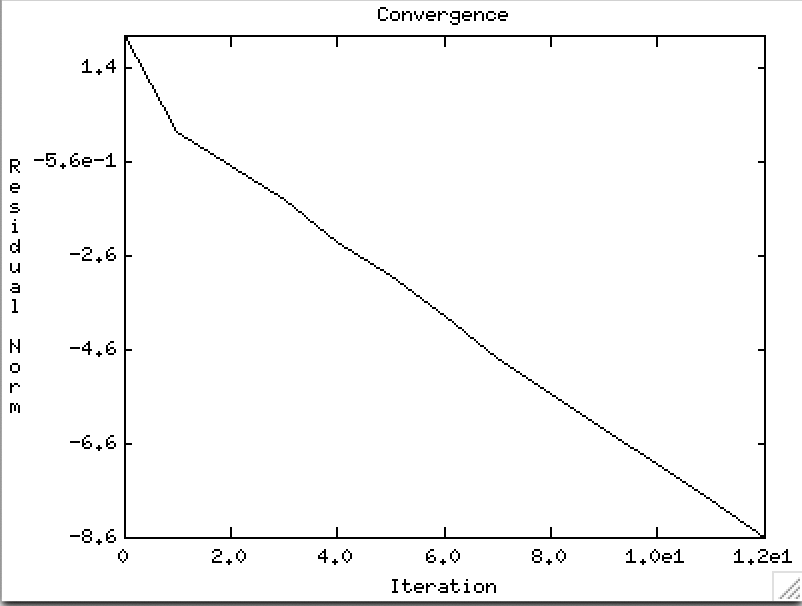
\includegraphics[width=2in]{figures/residualLG.png}\hfil
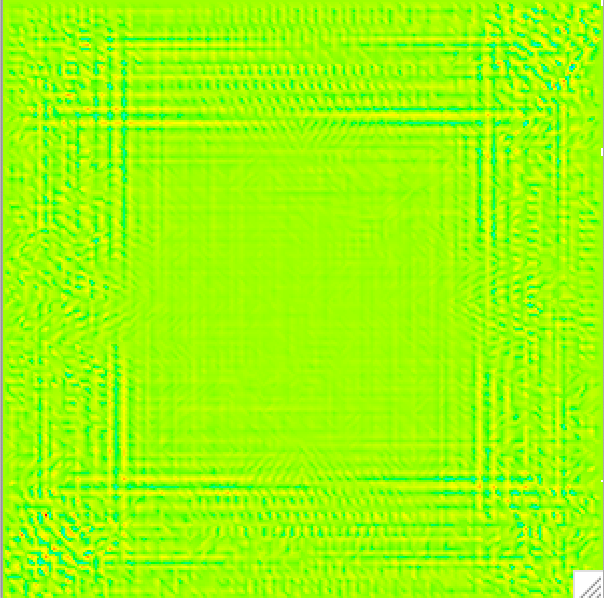
\includegraphics[width=2in]{figures/residualLast.png}
\caption{Plot of residual norm for each iterate of our multigrid solve on the left, and the residual itself for the last iterate on the right\label{fig:residualPlots}}
\end{figure}

The same sequence can be repeated for the error, since we are using MMS and can produce the exact solution. Using \bashinline{-ksp_monitor_error}, we produce the error norm for each iterate.
\begin{bash}
0 KSP Error norm 9.947802867762e-01
1 KSP Error norm 1.000114579455e-02
2 KSP Error norm 1.628832514084e-03
3 KSP Error norm 5.600031707378e-04
4 KSP Error norm 1.947734270258e-04
5 KSP Error norm 2.221932067247e-04
6 KSP Error norm 2.171843316734e-04
7 KSP Error norm 2.176959633670e-04
8 KSP Error norm 2.176494135621e-04
9 KSP Error norm 2.176509954453e-04
10 KSP Error norm 2.176519724470e-04
11 KSP Error norm 2.176516886193e-04
12 KSP Error norm 2.176517676049e-04
\end{bash}
Notice that the error stagnates well before we achieve convergence in the residual. This is because we hit the discretization error for our mesh. Refining the mesh will lower this bound, as we can see by running with \bashinline{-dm_refine_hierarchy 6},
\begin{bash}
0 KSP Error norm 9.993487701143e-01
1 KSP Error norm 1.232700481821e-02
2 KSP Error norm 2.400433256734e-03
3 KSP Error norm 4.230977361349e-04
4 KSP Error norm 6.442041832235e-05
5 KSP Error norm 1.421221753837e-05
6 KSP Error norm 2.668522964351e-06
7 KSP Error norm 3.579243209530e-06
8 KSP Error norm 3.382570470325e-06
9 KSP Error norm 3.409974576211e-06
10 KSP Error norm 3.408023096618e-06
11 KSP Error norm 3.407773635368e-06
12 KSP Error norm 3.407899220660e-06
\end{bash}
As before we can also run using \bashinline{-ksp_monitor_error draw::draw_lg} to generate a line graph of the above sequence, and \bashinline{-ksp_monitor_error draw} to plot the error over the domain, which are shown in Fig.~\ref{fig:errorPlots}. Notice that the error follows the structure of the solution, whereas the residual is much more oscillatory and seems not to be connected to the solution structure.

\begin{figure}
\centering
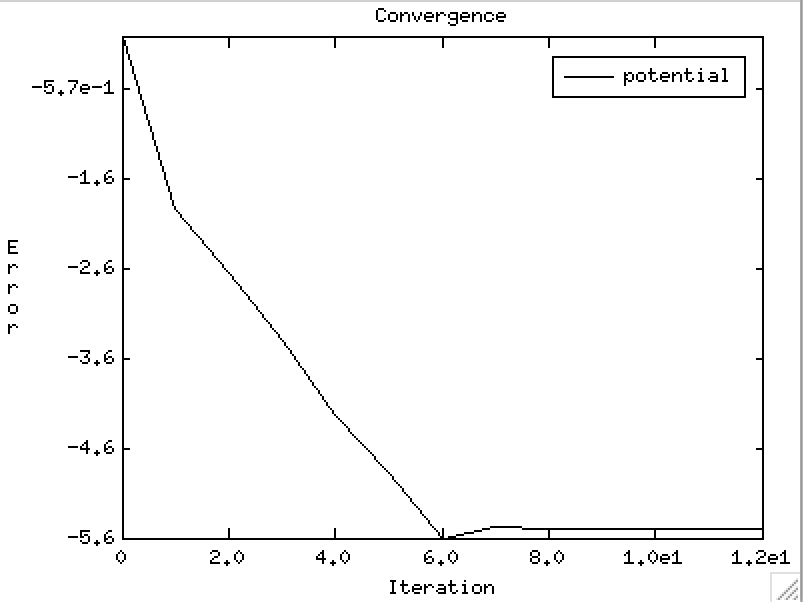
\includegraphics[width=2in]{figures/errorLG.png}\hfil
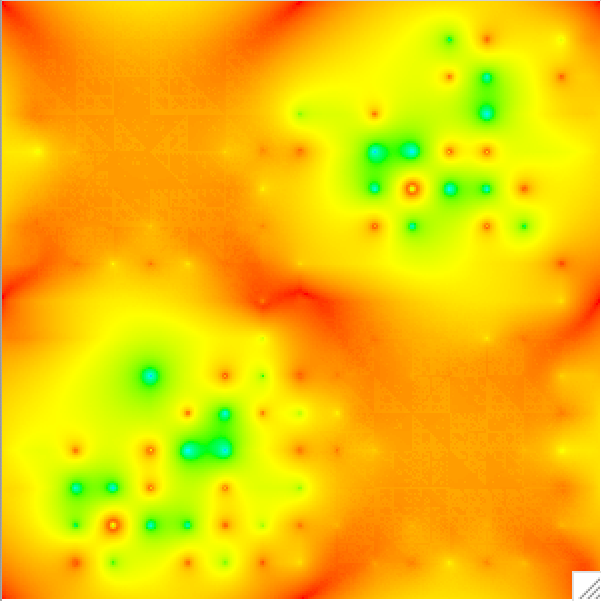
\includegraphics[width=2in]{figures/errorLast.png}
\caption{Plot of error norm for each iterate of our multigrid solve on the left, and the error itself for the last iterate on the right\label{fig:errorPlots}}
\end{figure}
